\section{Results}

\subsection{Epitope-tagged strain construction}

We developed a protocol for rapidly engineering the strains of the {\em Hb.} NRC-1 with epitope-tagged target proteins under the control of their native promoters. Using different classes of transcription factors, we demonstrate this approach's application and utility. In bacteria and archaea, different transcription factors may bind a wide span of target sites, ranging from one to hundreds. We chose to collect localization data from two extreme cases. The general transcription factor TfbD is known to bind hundreds of promoters \cite{facciotti_general_2007}. As an example of a specific regulator of a smaller regulon, we examined the Bat transcription factor. This transcription factor predicted to bind up to four potential sites and is one of the few haloarchaeal transcription factors with a well-described binding motif \cite{baliga_genomic_2001}.

Our epitope-tagging protocol for {\em Hb.} NRC-1 employed a homologous recombination method analogous to the gene deletion strategy developed by Peck {\em et al.} \cite{peck_homologous_2000}. This epitope knock-in strategy was described by Zhang et al. for ChIP-chip applications in human somatic cell lines \cite{zhang2008epitope}. For {\em tfbD}::HA strain construction, the novel vector pRSK01, which is compatible with Gateway ligation-independent cloning (Invitrogen, Carlsbad, CA), was created to facilitate and further standardize strain construction. This new vector allowed the use of either commercial DNA synthesis technology or PCR-mediated SOEing \cite{horton1989engineering} with Gateway compatible primers to rapidly construct the vectors used for strain construction. While in most instances PCR SOEing is still less expensive, the decreasing cost of DNA synthesis should make this approach a more attractive alternative for future large-scale strain construction projects.

{\em Hb.} NRC-1 $\Delta${\em pyrF} was transformed with a recombinant plasmid that contained the terminal 500bp of the target gene, a hemagglutinin (HA) tag, stop codon and 500bp downstream sequence (Figure \ref{SB_fig1}). Homologous recombination between the chromosomal target gene and the recombinant plasmid sequence introduced the HA tag to the chromosomal sequence. Successful first recombinants were determined by PCR screening of $\mathrm{Mev}^{\mathrm{R}}$ colonies ( Supplementary Figure S1 ). The plasmid was subsequently resolved using 5-FOA counter-selection as previously described \cite{kaur_systems_2006,peck_homologous_2000}. Strains with C-terminally HA-tagged target proteins were further verified by PCR and Sanger sequencing ( Supplementary Figures S1-S2 and Supplementary Information ). For the rapid construction of epitope-tagged transcription factor strains, this general strategy of utilizing DNA synthesis and homologous recombination-based chromosomal modification can be readily extended to any organisms with a system for targeted genetic knockouts.

\begin{figure}
\centering
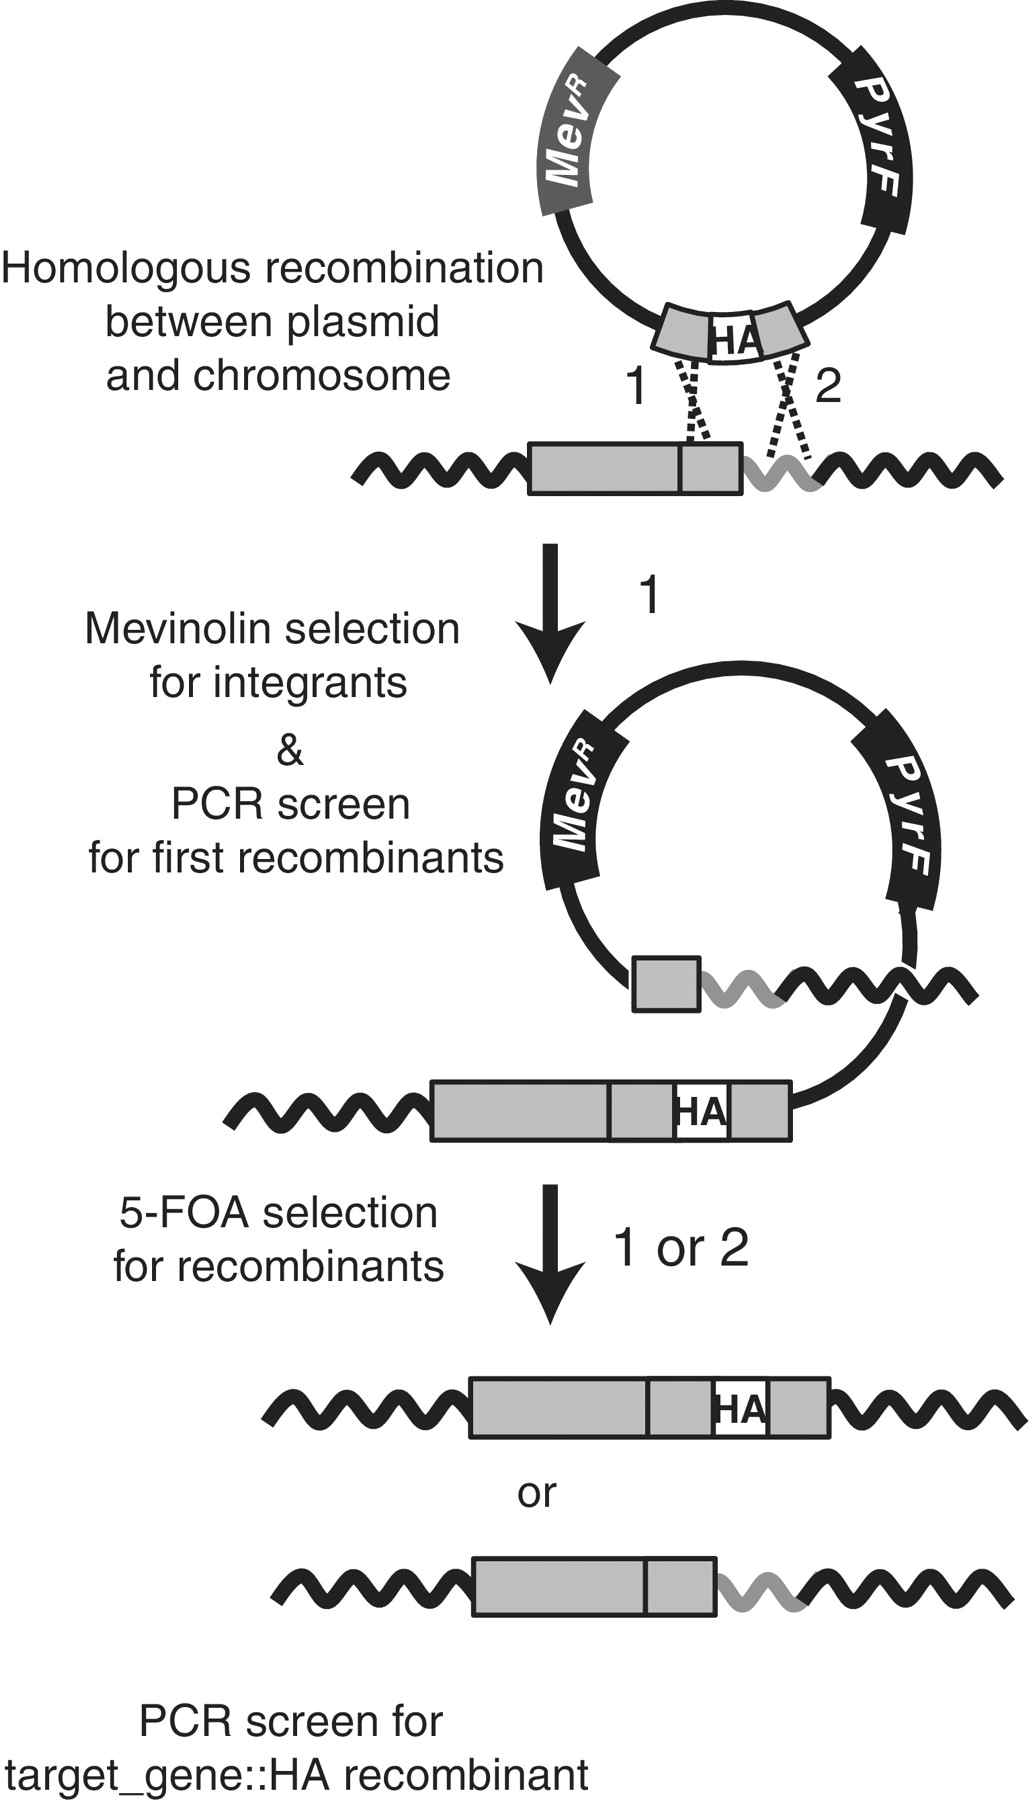
\includegraphics[width=20em]{SaltyBugs/figures/fig1}
\caption{Epitope tag-in approach for {\em Hb.} NRC-1. The {\em Hb.} NRC-1 $\Delta${\em pyrF} strain is transformed with a plasmid containing the mevinolin-resistance determinant ($\mathrm{Mev}^{\mathrm{R}}$ dark gray box) and the pyrF gene (black box) that confers 5-FOA sensitivity. The plasmid carries an engineered sequence containing the HA epitope sequence (white box) flanked by the last 500bp of the target gene and the 500bp downstream of the target gene (light gray boxes). Plasmid sequence is shown as solid line, chromosomal sequence is shown as solid, wavy lines. Cross-over can occur between target gene (light gray box) and flanking sequence (gray wavy line) in the chromosome and the homologous regions in the plasmid sequence, at either position 1 or 2 (position 1 example shown). PCR screening of mevinolin-resistant colonies is used to determine successful first recombinants. Subsequent plating on 5-FOA selects for second recombinants (via counter-selection with the {\em pyrF} gene). In this example, a second cross-over at site 2 produces the desired chromosomally integrated recombinant {\em target\_gene}::HA fusion. PCR screening of these colonies is required to distinguish this desired second recombinant from a second recombinant occurring at position 1. Drawing is not to scale.}
\label{SB_fig1}
\end{figure}

Western blotting with anti-HA antibody confirmed the specificity of the ChIP assay in these chromosomally tagged strains ( Supplementary Figure S3 ). The chromosomally integrated, epitope-tagged proteins remain under the control of their native promoters, as observed in the differential expression of the TfbD-HA protein over the course of growth in the recombinant strain $\Delta${\em pyrF} {\em tfbD}::HA ( Supplementary Figure S4 ). Increase in the abundance of TfbD during stationary phase is consistent with previous reports of tfbD transcriptional abundance \cite{facciotti2010large}. This approach can be used to monitor dynamic changes in the GRN that occur under different physiological conditions.

\subsection{Identifying target protein DNA-binding sites}

We used ChIP-seq to analyze with two different classes of target proteins: the general transcription factor TfbD and the Bat using recombinant strains that natively express the target protein ($\Delta${\em pyrF} {\em bat}::HA and $\Delta${\em pyrF} {\em tfbD}::HA). From the ChIP-seq datasets of 1.2 million reads for each factor, we identified 380 binding sites for TfbD and two binding sites for Bat (the {\em brp} and {\em crtB1} promoters).

These punctate target protein DNA-binding events produce a distinctive bimodal, strand-specific enrichment pattern in sequence coverage (Figure \ref{SB_fig2}). This enrichment pattern was leveraged to identify binding sites using our open source software package Pique, which reports the candidate binding site's enrichment as the ratio of sequence coverage in the IP data relative to a background control (Neches, R.Y., Wilbanks, E.G. and Facciotti, M.T., in preparation). Pique is implemented from a user-friendly graphical user interface and exports predicted binding sites to the Gaggle Genome Browser \cite{bare_integration_2010}. From the Gaggle genome browser, users can explore and curate the data before proceeding with analysis via other downstream Gaggle tools (Figure \ref{SB_fig3}).

\begin{figure}
\centering
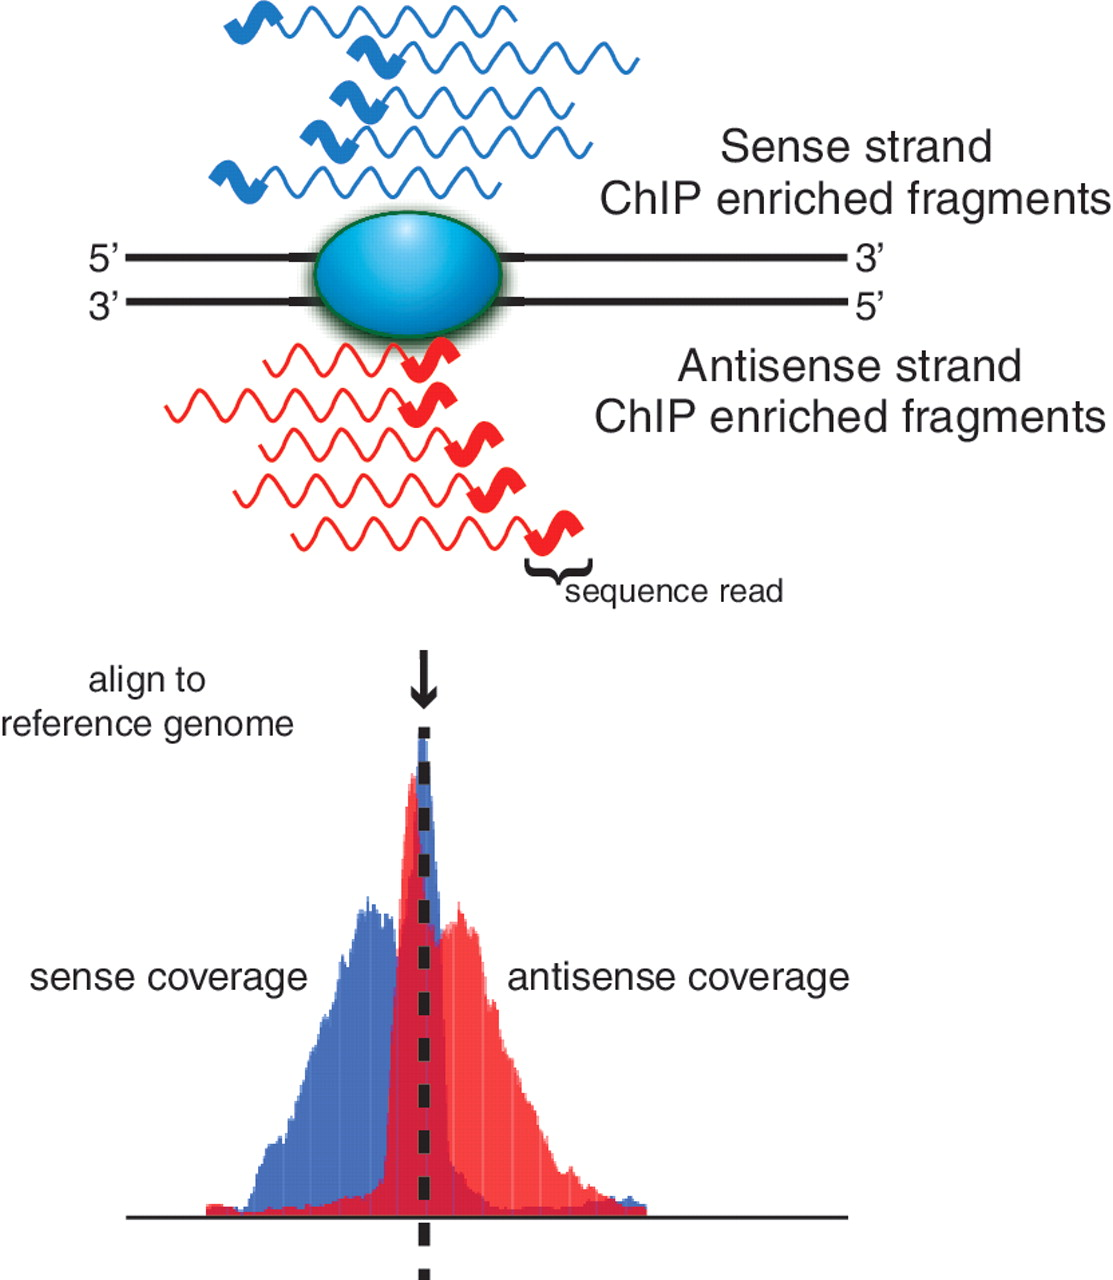
\includegraphics[width=20em]{SaltyBugs/figures/fig2}
\caption{The 5' to 3' sequencing requirement and short read length produce stranded bias in sequence coverage. The shaded blue oval represents the protein of interest bound to DNA (solid black lines). Wavy lines represent either sense (blue) or antisense (red) DNA fragments from ChIP enrichment. The thicker portion of the line indicates regions sequenced by short read sequencing technologies. Sequenced tags are aligned to a reference genome and shown below is the strand-specific sequence coverage at each position in the genome. Punctate-binding events (e.g. transcription factors) are characterized by well-defined strand-specific bimodality in sequence coverage.}
\label{SB_fig2}
\end{figure}


\begin{figure}
\centering
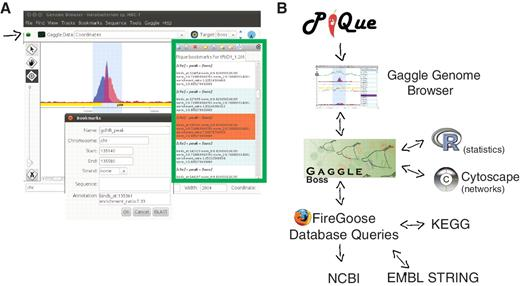
\includegraphics[width=20em]{SaltyBugs/figures/fig3}
\caption{The Pique software package processes ChIP-seq coverage data to predict protein-binding sites. Strand-specific coverage data are output as tracks for the Gaggle Genome Browser, and putative-binding sites (peaks) are output as `bookmark files.' (A) Screenshot of data browsing in the Gaggle Genome Browser. Green box outlines the navigation window for clicking through bookmarks of predicted binding sites. Details of each site can be displayed (inset). The Gaggle toolbar (shown with black arrow) can be used to broadcast selected data to other `geese' in the gaggle package, programs such as {\tt R}, {\tt cytoscape}, {\tt BLAST} or {\tt KEGG}. (B) Schematic overview of bioinformatics workflow.}
\label{SB_fig3}
\end{figure}

To confirm the specificity of the HA antibody for the ChIP assay on the recombinant HA-tagged strains, we conducted ChIP-seq on the $\Delta${\em pyrF} parent strain where no HA tags were expressed. The data contained a single peak, at chromosomal position 166589, likely because of the presence of a similar epitope in a native protein. This peak was present in all datasets examined and was subsequently filtered from all downstream analysis.

Independent biological replicates of the TfbD ChIP-seq experiment showed good reproducibility (82\% overlapping binding sites). Differences between the two replicates are due to the smallest peaks in each dataset, as indicated by examining increasingly stringent enrichment thresholds ( Supplementary Figure S5 ). Both binding sites in the Bat dataset and two example sites in the TfbD datasets (VNG906H and {\em atp\_p} promoters) were confirmed with a ChIP-qPCR assay. The relationship between the quantification of ChIP enrichment at the binding sites determined by qPCR and sequencing was found to be well correlated across several experiments (Figure \ref{SB_fig4}). The TfbD ChIP-seq binding sites agreed well with previously reported sites from TfbD ChIP-chip experiments \cite{facciotti_general_2007}. For both the ChIP-seq and ChIP-chip methods, 80\% of consensus binding sites from biological replicates were identified by at least one of the replicates from the other method.

\begin{figure}
\centering

\includegraphics[width=20em]{SaltyBugs/figures/fig4}
\caption{ChIP enrichment of binding sites determined by qPCR and sequencing show a linear relationship. Data shown are drawn from multiple ChIP experiments: the Bat ChIP (P {\em brp} and P {\em crtB1} closed and open circles) and the TfbD ChIP and the reduced cell number TfbD ChIPs (P VNG906H and P {\em atp\_p} ; closed and open triangles). Differences in enrichment at the TfbD-bound promoters corresponded to changes produced by decreasing the number of cells in the ChIP reaction (see \ref{SB_fig5} for further details).}
\label{SB_fig4}
\end{figure}

\subsection{Spatial resolution}

The spatial resolution of the ChIP-seq binding site prediction was assessed for the Bat and TfbD datasets. As the Bat transcription factor has a well-characterized predicted binding motif \cite{baliga_genomic_2001}, we used the distance from our predicted binding site to the motif center as an estimate of the spatial resolution. The binding sites at the {\em brp} and {\em crtB1} promoters were found, respectively, at 20 and 27bp upstream of the predicted Bat-binding motif center (3' displaced).

As there exists no well-defined binding motif for the general transcription factor TfbD, we used proximity to the nearest predicted transcript start site (TSS) as a measure of spatial resolution for this factor. Archaeal TFB proteins, homologs of the eukaryotic factor TFIIB, canonically bind at B-recognition elements $\sim$30-50bp upstream of the TSS, in association with a TATA-binding protein \cite{bell_transcription_1998}. Eighty-six percent of the 312 consensus binding sites from the TfbD ChIP-seq biological replicates were found within 250bp of a predicted TSS (in either 3' or 5' direction). We measured the distance from each of these predicted binding sites to the nearest predicted TSS. These values were compared to the distance to TSS from previously reported TfbD ChIP-chip sites, determined with both 500-bp contiguous and 12-bp overlapped tiling microarray (Figure \ref{SB_fig5}) \cite{facciotti_general_2007}. The distance to TSS for the ChIP-seq binding sites (median=32, mean=51) is in agreement with the expected binding pattern for this general transcription factor, and is significantly smaller than that predicted by both resolutions of ChIP-chip microarray (Mann Whitney U-test, $p$ value $<0.005$). The variance in these distance measurements provides an estimate of the precision with which each method maps binding sites. The ChIP-seq dataset has significantly decreased variance relative to both ChIP-chip datasets (significance assessed by Bartlett test, $p$ value $<0.005$; samples were tested for normality by two-sided Kolmogorov-Smirnov $p$ value $<0.0005$). Taken together, these data indicate that the ChIP-seq assay offers improved spatial resolution in mapping the target protein-binding site relative to prior ChIP-chip assays.

\begin{figure}
\centering
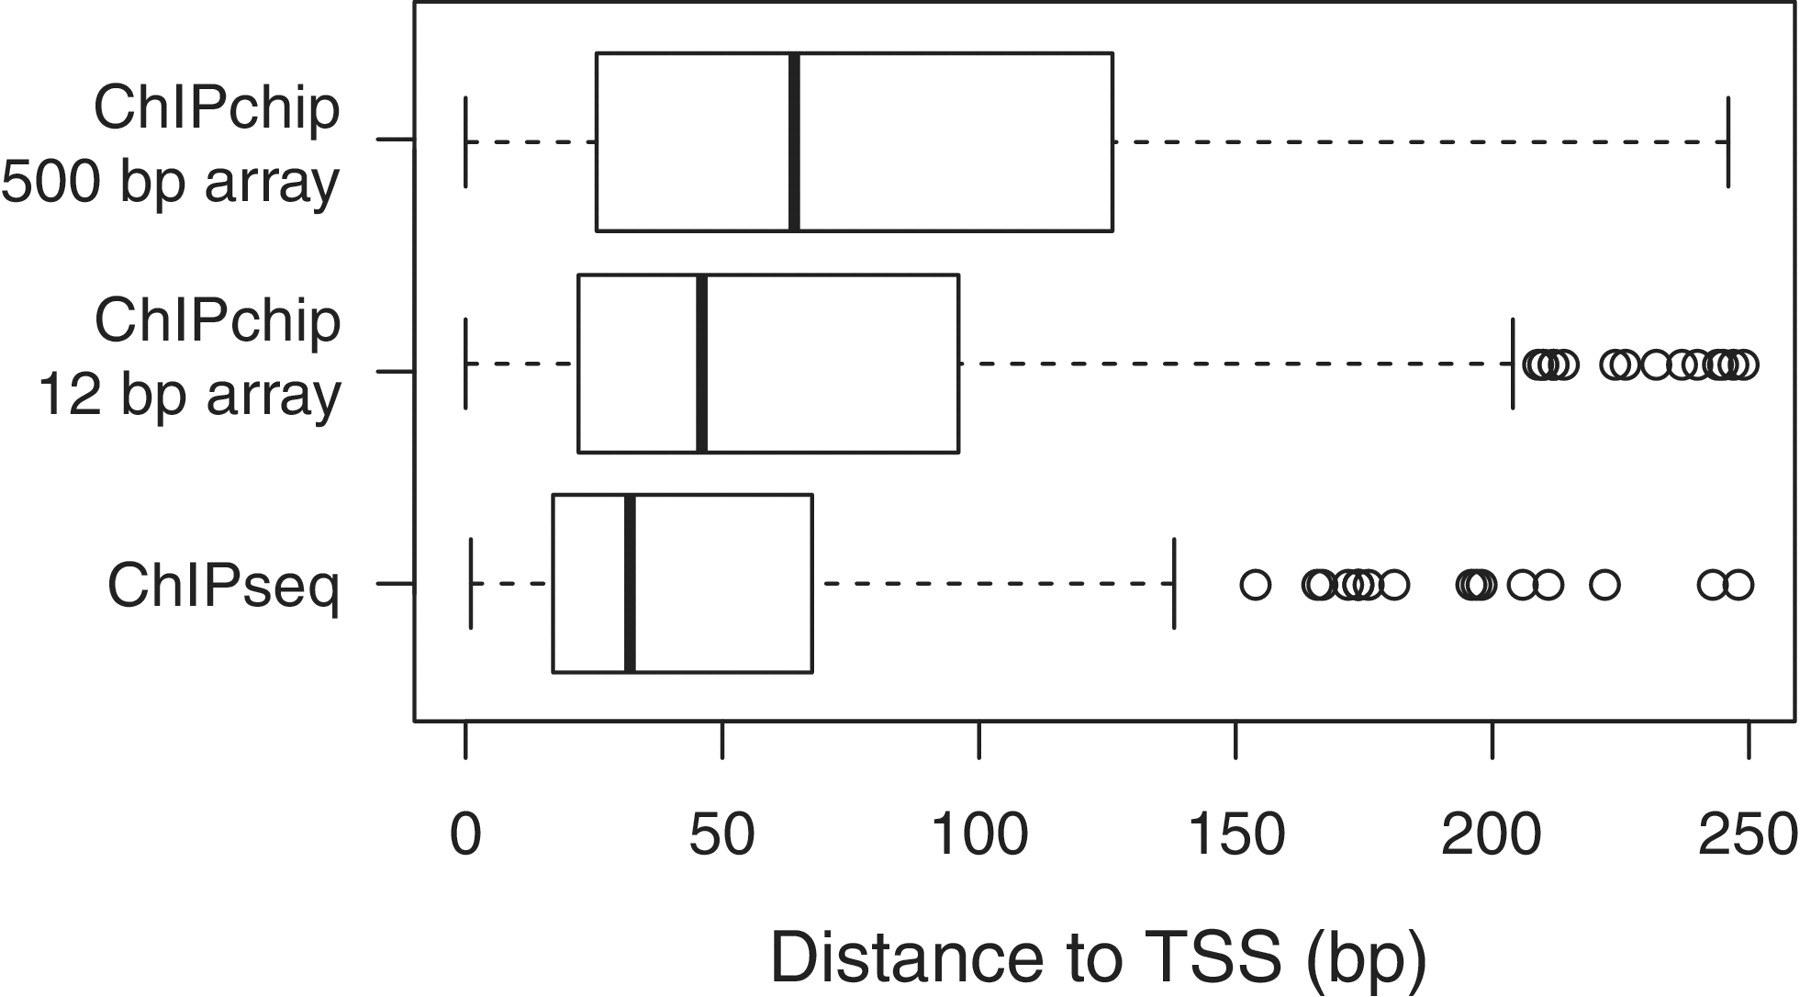
\includegraphics[width=20em]{SaltyBugs/figures/fig5}
\caption{Distance from predicted TfbD-binding site for ChIP-seq (consensus between biological replicates), 500-bp tiling microarray ChIP-Chip (consensus between biological replicates) and 12-bp tiling microarray ChIP-Chip experiments. The observed difference in means was statistically significant (Mann Whitney U-test, p value $<0.005$), as is the observed difference in variance (Bartlett test, p value $<0.005$).}
\label{SB_fig5}
\end{figure}

\subsection{ChIP assay cell number and sequencing depth}

We investigated the number of cells required for ChIP to produce sufficient enrichment at target protein-binding sites. Decreasing the number of cells in the ChIP reaction lowered the observed enrichment at target protein-binding sites; however, enrichment ($>5\times$) was detectable for highly enriched TfbD-binding sites when as few as $3.50 \times 10^8$ cells were used for ChIP, equivalent to 1 ml of a typical culture (Figure \ref{SB_fig6}A). Because of the overall decrease in enrichment, smaller cell number ChIPs were less sensitive in binding site detection but maintained specificity (Figure \ref{SB_fig6}B). The relatively small volume required for this ChIP assay should enable the high-throughput application of this method in the context of dynamic binding studies by allowing for the repetitive sampling of numerous strains with minimal perturbation.

\begin{figure}
\centering
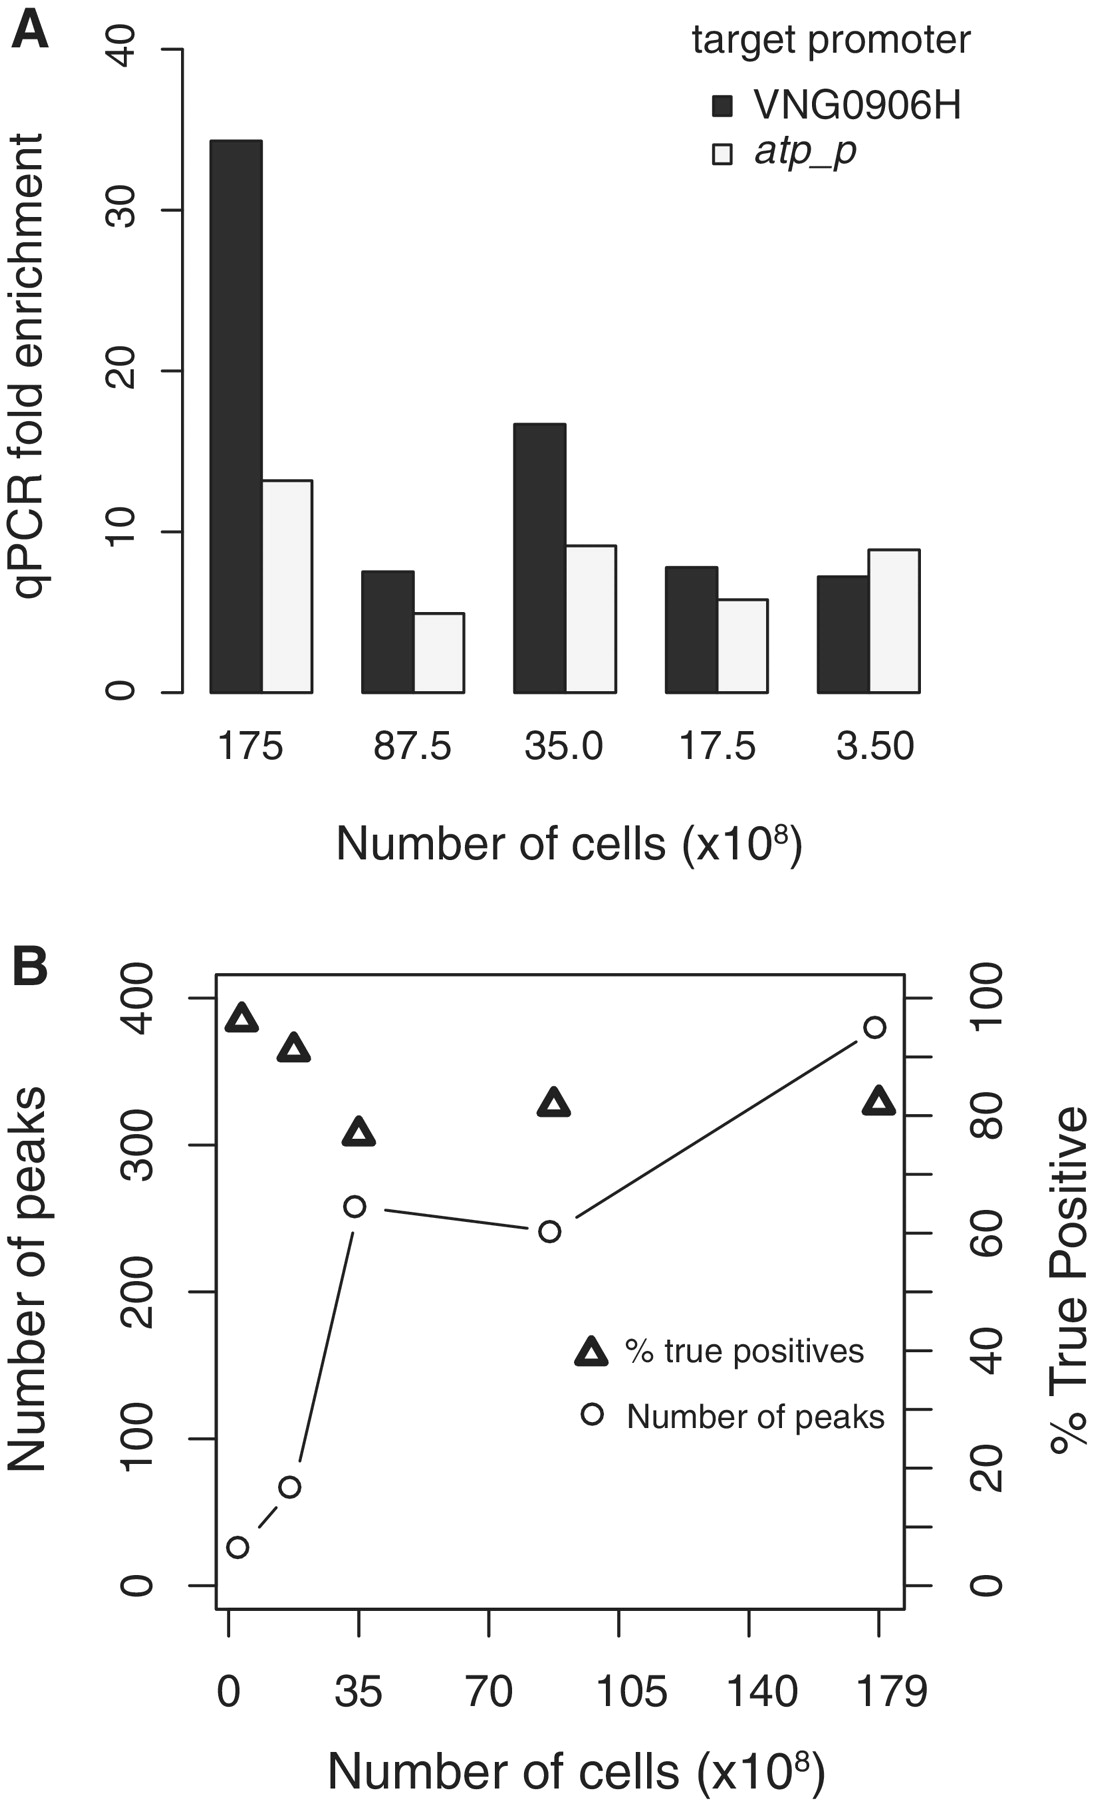
\includegraphics[width=20em]{SaltyBugs/figures/fig6}
\caption{TfbD ChIP with decreasing numbers of cells. \textbf{A.} ChIP-qPCR determined fold enrichment at two test promoters (VNG906H, dark bars and {\em atp\_p} light bars) decreases with lower numbers of cells; however, strong ($>5\times$) enrichment is still observed with $3.5 \times 10^8$ cells. \textbf{B.} For decreasing cell volume ChIP-seq experiments, fewer peaks could be identified (number of peaks identified, squares and lines), resulting in a significant loss in sensitivity. However, the percentage of identified peaks that were true positives stayed high (\% true positives, triangles). True positives were defined as binding sites that were shared with at least one of the optimized $1.75 \times 10^{10}$ ChIP TfbD biological replicates.}
\label{SB_fig6}
\end{figure}

One of the main advantages to the ChIP-seq platform for small microbial genomes is the ability to decrease the experimental cost by multiplexing many samples in a single sequencing lane. We carried out an {\em in silico} analysis to determine the depth of sequencing necessary to achieve sensitive and accurate detection of binding sites. Sequence reads were randomly subsampled to decreasing coverage levels from 1.2M reads ($15.4\times$ coverage) to 10000 reads ($0.13\times$ coverage). For the TfbD dataset, the number of peaks identified remained stable down to 500K reads ($5\times$ coverage), after which the sensitivity began to decrease (Figure \ref{SB_fig7}). The specificity of binding site identification remained excellent below 500K reads, even though the sensitivity decreased (Figure \ref{SB_fig7}).

\begin{figure}
\centering
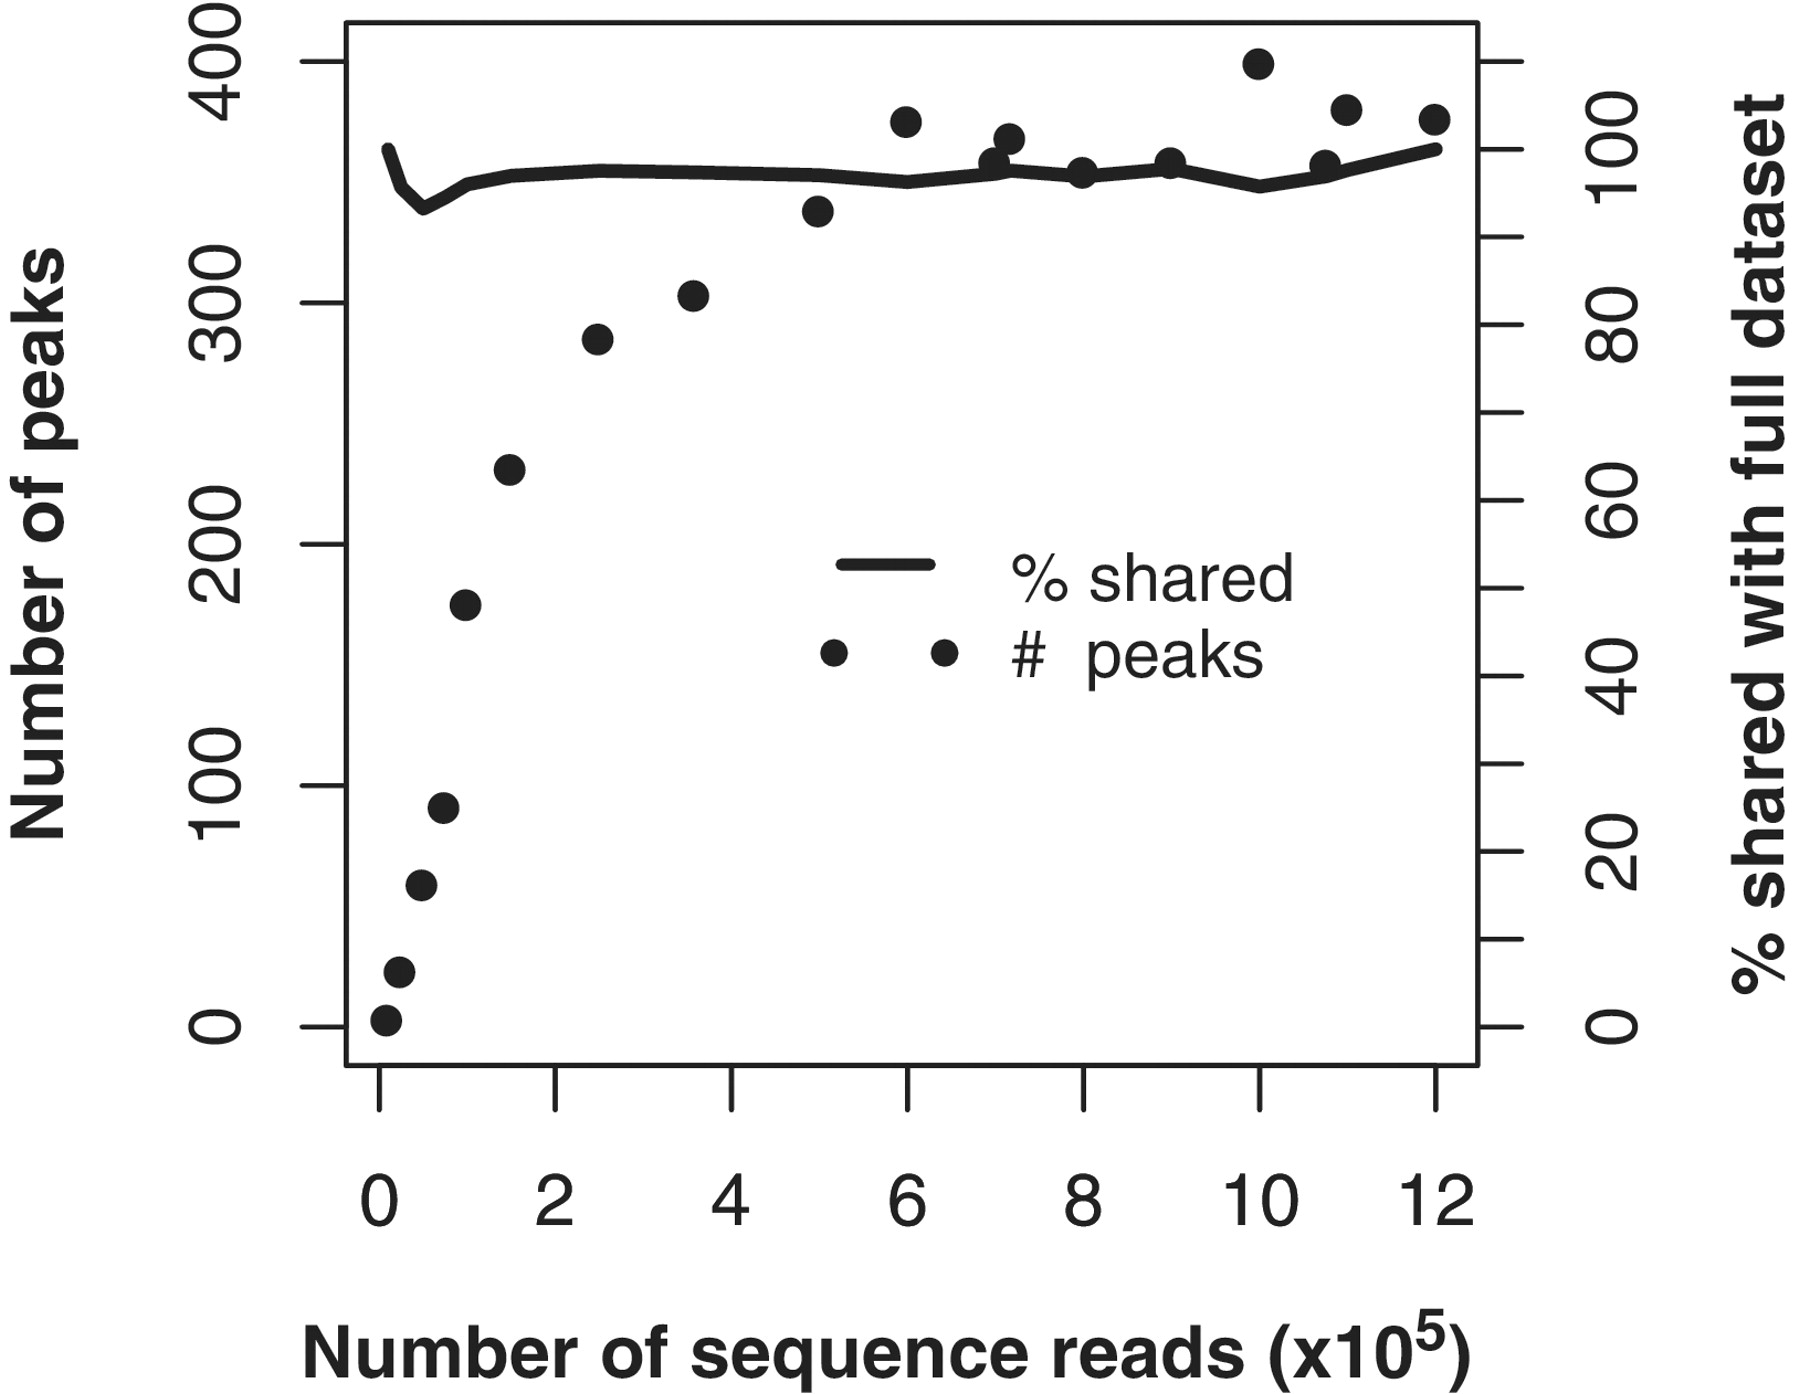
\includegraphics[width=20em]{SaltyBugs/figures/fig7}
\caption{Subsampling sequence coverage. Sequences were randomly sampled from a TfbD ChIPseq dataset of 6M reads to create subsampled datasets of decreasing coverage. The number of peaks that could be identified in each subset (filled circles) is shown as a function of the number of sequence reads in the dataset. The specificity of these smaller lists is assessed as the percentage of the identified peaks which overlapped the larger 1.2M read dataset (solid line).}
\label{SB_fig7}
\end{figure}

For the Bat dataset, the more strongly enriched binding site at the {\em brp} promoter could be detected in datasets as small as 50000 reads ($0.64\times$ coverage), whereas the weaker binding at the {\em crtB1} promoter was undetectable below 150000 reads ($1.9\times$ coverage). No false positives were detected in these lower coverage datasets, with the exception of a single site in the 200000 read dataset. Examining the effect of decreased coverage on the spatial resolution, we found that the automated prediction of the binding site remained accurate, until just before the site became undetectable (Figure \ref{SB_fig8}).


\begin{figure}
\centering
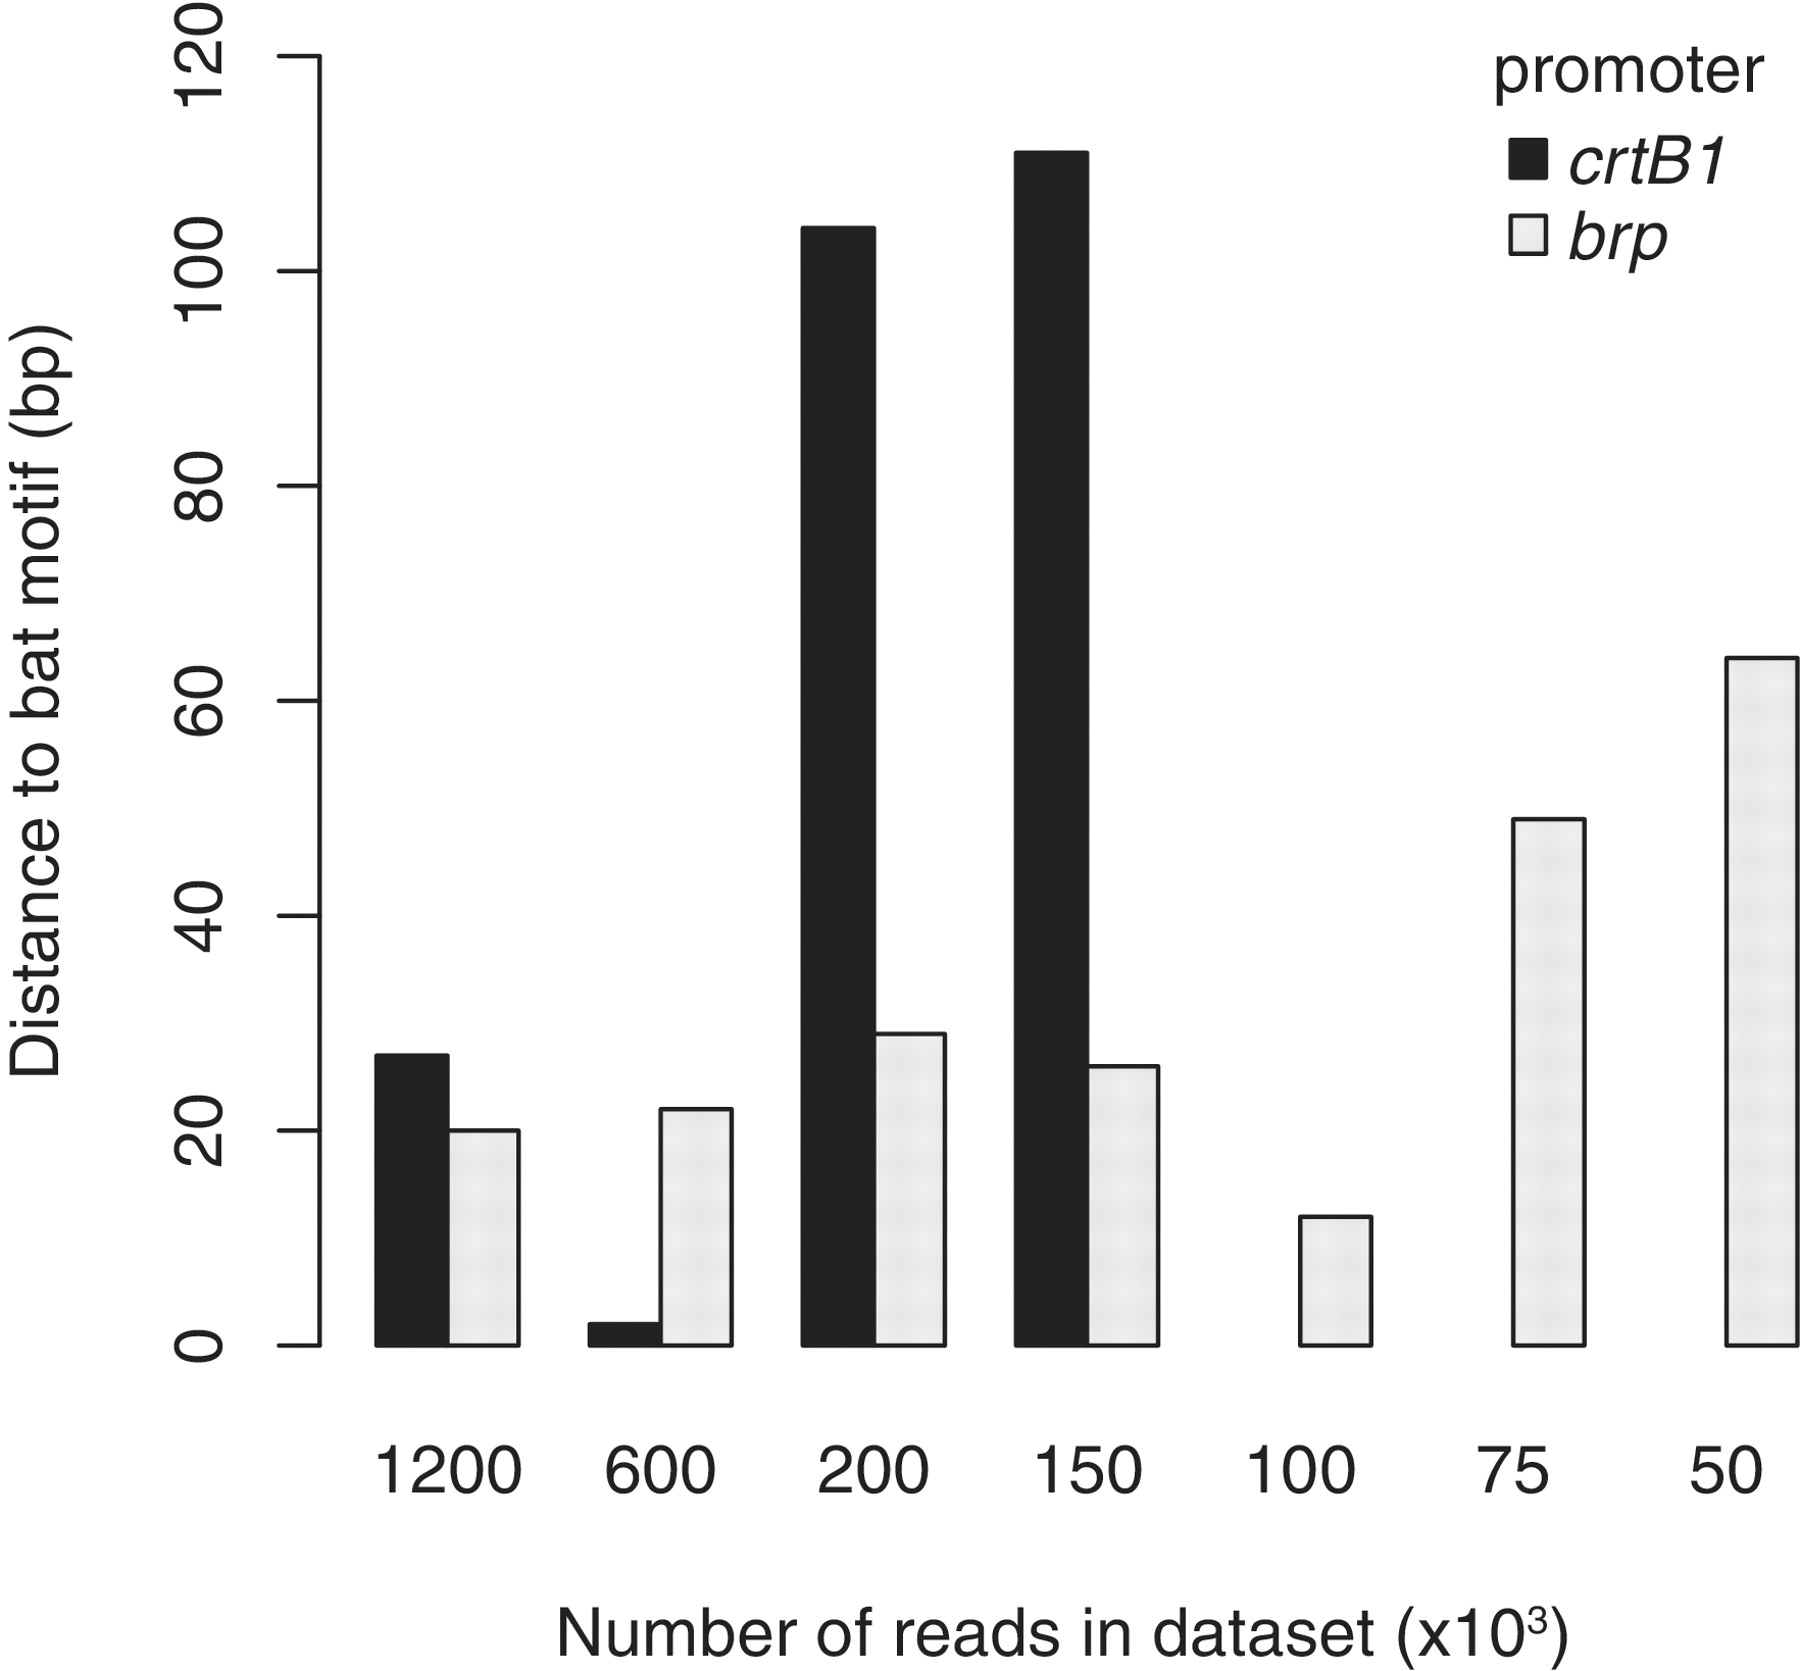
\includegraphics[width=20em]{SaltyBugs/figures/fig8}
\caption{Spatial resolution of binding sites calculated from randomly subsampled Bat ChIP-seq datasets of decreasing coverage. The distance from ChIPseq predicted binding site to nearest Bat-binding motif was calculated for both the {\em crtB1} (dark gray bars) and {\em brp} (light gray bars) promoter regions. Binding sites for in the {\em crtB1} promoter could not be detected for datasets with 100000 reads and below (no bars in plot).}
\label{SB_fig8}
\end{figure}
